\documentclass[12pt]{article}
\usepackage{geometry}
\geometry{
	left=20mm,
	top=20mm,
}
\usepackage[utf8]{inputenc}
\usepackage[shortlabels]{enumitem}
\usepackage{array}
\newcolumntype{C}[1]{>{\centering\let\newline\\\arraybackslash\hspace{0pt}}m{#1}}
\usepackage[spanish,es-nodecimaldot]{babel}
 \usepackage{url}
\usepackage[spanish, fixlanguage]{babelbib}
\bibliographystyle{IEEEtran}
\usepackage{graphicx}
\graphicspath{ {./images/} }
\usepackage{amssymb}
\usepackage{amsmath}
\usepackage{subcaption}
\usepackage[linesnumbered]{algorithm2e}
\newcommand\mycommfont[1]{\footnotesize\ttfamily\textcolor{blue}{#1}}
\SetCommentSty{mycommfont}
\usepackage{tikz}
\usetikzlibrary{positioning, fit}
\usetikzlibrary{babel}
\usepackage{titlesec}
\titlespacing*{\section}
{0pt}{5.5ex plus 1ex minus .2ex}{.3ex plus .1ex}
\titlespacing*{\subsection}
{0pt}{5.5ex plus 1ex minus .2ex}{2.3ex plus .1ex}
\title{Tarea 8}

\author{
	Saul Ivan Rivas Vega \\
	\\
	Diseño y análisis de algoritmos\\
\\
	Equipo Completo:\\
		Yadira Fleitas Toranzo\\
		Diego de Jesús Isla Lopez\\
		Saul Ivan Rivas Vega\\
}

\date{\today}

\begin{document}
	\maketitle
	\pagebreak
	\section{Ejercicio 1.}
	\paragraph{} Considera el siguiente problema de \textit{formato de textos}. Como entrada tenemos un arreglo $W[1,...,n]$ tal que cada $W[i]$ es una palabra; supondremos que el último símbolo en $W[i]$ es un espacio en blanco.También recibimos un entero \textbf{long\_linea} $> 0$ como parte de la entrada, tal que \textbf{long\_linea} es mayor o igual a la longitud de cada palabra $W[i]$, denotada $|W[i]|$. Lo que buscamos es dar \textit{fomato} al texto en $W$ para esto hay que decidir cuales palabras van juntas en la misma línea. Si decidimos poner en una misma línea las palabras $W[i],...,W[i']$, $i\leq i'$, lo que se denota $l[i,i']$, entonces la \textit{penalización} de $l[i,i']$ es:
	\begin{itemize}
		\item $\infty$ si \textbf{long\_linea} $< |W[i]| + ... + |W[i']|$ (es decir, las palabras no caben en una sola línea);
		\item de otra forma, $($\textbf{long\_linea}$-(|W[i]| + ... + |W[i']|))^3$
	\end{itemize}
	Entonces, la \textit{penalización} de un \textit{formato} $l_1[1,i_1], l_2[i_1+1, i_2], ..., l_j[i_{j-1}+1, n]$ de $W$ es la suma de las penalizaciones de sus líneas.
	 \\
	 \subsection{a) Demuestra que la siguiente estrategia \textit{greedy} produce \textit{formatos} arbitrariamente malos, es decir, con penalizaciones arbitrariamente grandes}
	 \paragraph{}Procesamos las palabras de $W[1]$ a $W[n]$; si aún hay espacio suficiente para meter $W[i]$ en la línea actual, entonces la metemos; de otra forma iniciamos una nueva línea en la que ponemos a $W[i]$.
	 \paragraph{Demostración.} Podemos demostrarlo dando un ejemplo donde esto sucede.\\
	 Sea $n=3$, $long\_linea=6$ y con las longitudes 
	 $|W[1]|=3$, $|W[2]|=3$ y  $|W[3]|=2$.\\
	 \begin{itemize}
	 	\item El algoritmo tomará la línea actual con espacio disponible de $6$ y procesará la primera palabra, $W[1]$.
	 	\item Como el espacio disponible es $6$ y $|W[1]|=3$ entonces la metemos en la línea actual.
	 	\item Ahora el espacio disponible es $3$ y como $|W[2]|=3$ entonces la metemos en la línea actual.
	 	\item Como el espacio disponible es $0$ y $|W[3]|=2$ creamos una nueva linea y metemos a $W[3]$ en ella.
	 \end{itemize}
 	Al terminar el algoritmo terminamos con un formato $f_1$ con las lineas $l_1[1,2]$ y la linea $l_2[3, 3]$. Veamos sus \textit{penalizaciones}.\\
 	En el caso de $l_1[1,2]$, $|W[1]|+|W[2]|$ es igual a $long\_linea$ entonces entra en el segundo caso de la función de \textit{penalización} entonces la calculamos con: 
 	\begin{equation}
 		\begin{split}
 		\textit{penalizacion}(l_1[1,2])= & (long\_linea - (|W_1| + |W_2|))^3 \\
 		 = & (long\_linea - (3 + 3))^3 \\
 		 = & (long\_linea - 6)^3\\
 		 = & (6 - 6)^3\\
 		 = & (0)^3 \\
 		 = & 0
 		\end{split}
 	\end{equation}
	Para $l_2[3,3]$, $|W[3]|$ es menor a $long\_linea$ entonces entra en el segundo caso de la función de \textit{penalización} entonces la calculamos con: 
	\begin{equation}
	\begin{split}
	\textit{penalizacion}(l_2[3,3])= & (long\_linea - (|W_3|))^3 \\
	= & (long\_linea - (2))^3 \\
	= & (long\_linea - 2)^3\\
	= & (6 - 2)^3\\
	= & (4)^3 \\
	= & 64
	\end{split}
	\end{equation}
	Ahora la \textit{penalización} del formato $f_1$ es la suma de las dos penalizaciones de sus líneas:
	\begin{equation}
		\textit{penalización $f_1$}= 64 + 0 = 64 
	\end{equation}
	Sin embargo, tomemos el siguiente formato $f_2$ con las líneas, $l_1[1,1]$ y $l_2[2,3]$. Para $l_1[1,1]$ tenemos:
	\begin{equation}
	\begin{split}
	\textit{penalizacion}(l_1[1,1])= & (long\_linea - (|W_1|))^3 \\
	= & (long\_linea - (3))^3 \\
	= & (long\_linea - 3)^3\\
	= & (6 - 3)^3\\
	= & (3)^3 \\
	= & 27
	\end{split}
	\end{equation}
	Y para $l_2[2,3]$ tenemos:
	\begin{equation}
	\begin{split}
	\textit{penalizacion}(l_2[2,3])= & (long\_linea - (|W_2|+|W_3|))^3 \\
	= & (long\_linea - (3 + 2))^3 \\
	= & (long\_linea - 5)^3\\
	= & (6 - 5)^3\\
	= & (1)^3 \\
	= & 1
	\end{split}
	\end{equation}
	Por lo tanto la \textit{penalización} total para el formato $f_2$ es:
	\begin{equation}
	\textit{penalización $f_2$}= 27 + 1 = 28 
	\end{equation}
	Finalmente como $f_1$ es mayor que $f_2$ y además podemos formar arreglos agregando las mismas 3 longitudes del ejemplo en ese orden decimos que el algoritmo produce \textit{formatos} con penalizaciones arbitrariamente grandes.
	\subsection{b) Usa la técnica de programación dinámica para diseñar un algoritmo que encuentre un formato con penalización mínima. Demuestra la correctitud de tu algoritmo y haz un análisis de tiempo y espacio.}
	\subsection{c) Modifica tu algoritmo para que funcione con una función de penalización de línea dada; la penalización de un formato sigue siendo la suma de las penalizaciones de sus líneas.}
\section{Ejercicio 2}
	\paragraph{} Considera un arreglo $A[1,...,n]$ con enteros positivos en sus entradas. Decimos que una pareja $(i,j)$ es un \textit{declive} si $i\leq j$ y $A[i]\geq A[j]$; la \textit{longitud} de $(i,j)$ es $A[i] - A[j]$. Diseña un algoritmo de tiempo y espacio $o(n^2)$ que calcule un declive de $A$ de longitud máxima (es $o$ pequeña, investiga ese concepto). Demuestra que tu algoritmo es correcto y haz el análisis de tiempo y espacio.\\
	\begin{algorithm}[H]
		\KwData{Arreglo $A$.}
		\KwResult{Tupla $(max\_long, r\_i, r\_j)$ Que representa el valor de la longitud máxima de un declive en $A$ y los índices $r\_i,r\_j$ de dicho declive $(r\_i,r\_j)$.}
		\SetAlgoLined
		\tcc{Inicializamos una cola de prioridad donde guardaremos tuplas $(A[i], i)$ donde ordenaremos mayor a menor por $A[i]$.}
		$Q=\{\}$\;
		\tcc{Inicializamos las respuestas actuales.}
		$max\_long=-\infty$\;
		$r\_i=0$\;
		$r\_j=0$\;
		\tcc{Recorremos del final al inicio el arrego $A$, pasando por todas las posiciones desde $n$ hasta $1$.}
		\For{i = n, i $\geq$ $1$}{
			\tcc{Insertamos el elemento actual a la cola de prioridad.}
			$(A[i], i)\rightarrow Q$\;
			\tcc{Obtenemos el elemento al frente de $Q$, es decir la tupla $(A[i], i)$ con menor $A[i]$, no lo removemos de la cola de prioridad solo obtenemos sus valores.}
			$(valor, indice)\leftarrow Q$\;
			\tcc{Como procesamos de fin a inicio este elemento cumple que $i \leq indice$, ahora entonces revisamos si $A[i]\geq valor$ lo cual sería un declive $(i, indice)$.}
			\If{$A[i]\geq valor$}{
				\tcc{Calculamos la longitud del declive $(i, indice)$.}
				$current\_long = A[i] - valor$\;
				\tcc{Actualizamos nuestra respuesta si es mayor a la que llevabamos.}
				\If{$current\_long > max\_long$} {
					$max\_long = current\_long$\;
					$r\_i=i$\;
					$r\_j=indice$\;
				}
			}
		}
		return ($max\_long, r\_i, r\_j$)\;
		\caption{Algoritmo MAXDECLIVE.}
	\end{algorithm}
\subsection{Demostración correctitud.}
\paragraph{El algoritmo termina.} El algoritmo termina puesto que solo realiza un loop con $n$ iteraciones en las cuales se realizan asignaciones y comparaciones que podemos asumir de tiempo constante, sin embargo también se realizan inserciones en una cola de prioridad que como hemos revisado anteriormente, son de tiempo $logn$. Por lo tanto podemos decir que el algoritmo termina después de $n$ iteraciones, posteriormente en el análisis temporal desarrollaremos la complejidad de cada iteración.
\paragraph{El algoritmo devuelve un declive de longitud máxima.}
Podemos partir de explicar cuál es un algoritmo que por fuerza bruta encuentra la respuesta. Es un algoritmo que solo intentará todas las posibles parejas $i,j$ donde $i\leq j$ y verificará si es un declive, conservando el declive con longitud máxima, lo cuál sería de tiempo $O(n^2)$ lo cual no cumple con nuestra restricción temporal de $o(n^2)$. Sin embargo tomemos la siguiente observación.
\paragraph{Observación 1} No es necesario revisar todos los $j$ tales que $j \geq i$ para encontrar un declive de longitud máxima que tiene a $i$ como primer elemento, solo es necesario revisar al elemento $j$ tal que $j \in [i,...,n]$ y además tenga el menor valor en $A[i,...,n]$. 
\paragraph{Demostración de la Observación 1} Por contradicción.\\
Supongamos que el declive de longitud máxima que tiene a $i$ como primer elemento no es con el $j$ tal que $j \in [i,...,n]$ y además tenga el menor $A[j]$, sino con un $j'$ tal que por lo menos cumple que $j' \in [i,...,n]$ y además $A[j] \leq A[i]$ para ser un declive. Si $j'$ tiene el menor valor en $A[i,...,n]$ entonces significa que $j' = j$, en otro caso significa que $A[j]< A[j']$, y podemos desarrollar la siguiente ecuación:
\begin{equation}
	\begin{split}
	A[j]< A[j']\\ 
	-A[j]> -A[j']\\
	A[i]-A[j]> A[i]-A[j']\\
	\end{split}
\end{equation}
Lo cual significa que la longitud del declive tomando al elemento $j$ es mayor al declive tomando al elemento $j'$, pero esto es una contradicción puesto que en la suposición inicial el declive $(i, j')$ era el de longitud máxima.
Finalmente como no puede existir dicho $j'$ decimos que el declive de longitud máxima que tiene como primer elemento a $i$ es $(i,j)$ donde el elemento $j$ cumple que $j \in [i,...,n]$ y además tiene el menor valor en $A[i,...,n]$
\paragraph{} Ahora tomando la \textbf{Observación 1} podemos demostrar la correctitud del algoritmo por contradicción.
Supongamos que el declive de longitud máxima $(i',j')$ no fue devuelto por el algoritmo. Por la \textbf{Observación 1} para dicho declive significa que $j'$ cumple que $j' \in [i',...,n]$ y además tiene el menor valor en $A[i',...,n]$. El algoritmo debió haber ignorado a $i'$ puesto que para cuando se encuentra en el índice $i$ justamente revisa el elemento $j$ tal que cumple que $j \in [i,...,n]$ y además tiene el menor valor en $A[i,...,n]$. Sin embargo, el algoritmo si revisa todos los índices $1 \leq i \leq n$ pero esto es una contradicción puesto que no puede haber revisado e ignorado al índice $i'$. Finalmente decimos que el algoritmo devuelve un declive de longitud máxima.
\subsection{Análisis de tiempo}
\paragraph{El algoritmo es de complejidad $O(nlogn)$ y por lo tanto $o(n^2)$} Como vimos en la sección donde se explicaba que el algoritmo termina, el algoritmo solo realiza un loop de fin a inicio por los $n$ elementos en $A$, sin embargo en cada iteración además de las operaciones de asignación y comparación que podemos asumir de tiempo $O(1)$, también tenemos operaciones de inserción y consulta a una cola de prioridad que como anteriormente hemos visto son de complejidad $O(logn)$. Por lo tanto el algoritmo es de complejidad $O(nlogn)$ y como para toda constante $c>0$ existe un $n_0$ tal que para toda $n\geq n_0$ se cumple que $nlogn < n^2$ decimos que el algoritmo es $o(n^2)$.
\subsection{Análisis de espacio}
\paragraph{El algoritmo ocupa espacio de orden $O(n)$} 
Adicional a la entrada el algoritmo ocupa algunas variables individuales para las respuestas y consultar a la cola de prioridad las cuales podemos considerar de orden $O(1)$. Sin embargo también hacemos uso de una cola de prioridad y adicionalmente no removemos los elementos que insertamos en ella y como cada elemento es una pareja, tendremos al final $2n$ valores en la cola de prioridad. Como $2n$ es el factor dominante decimos que el algoritmo tiene espacio de orden $O(2n)$ y finalmente $O(n)$.
\section{Ejercicio 3}
	\paragraph{} Considera el problema de selección de centros visto en clase. Demuestra que el siguiente algoritmo devuelve un conjunto $C$ con a lo más $k$ centros tal que $rc(C)\leq 2rc(C^*)$, donde $C^*$ es un conjunto con a lo más $k$ centros óptimo, es decir con radio de covertura mínimo. Puedes suponer como correctos todos los algoritmos y afirmaciones vistas en clase.
	\begin{figure}[h]
		\begin{center}
			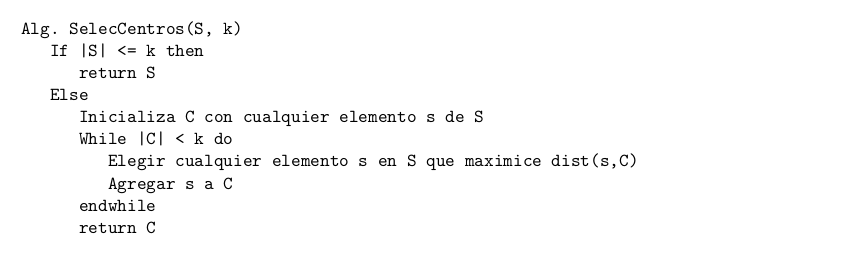
\includegraphics[width=\textwidth]{AlgCentros}
		\end{center}
	\end{figure}
\pagebreak
\section{Ejercicio 4}
\paragraph{} Escribe una versión recursiva del algoritmo probabilístico de corte mínimo visto en clase (basado en contracciones de aristas). Demuestra que el conjunto de aristas devuelto por el algoritmo es efectivamente un corte de la gráfica inicial.
\section{Ejercicio 5}
\paragraph{} Tenemos $n$ servidores que buscan coordinarse para ejecutar localmente la misma acción. De forma \textit{abstracta}, los servidores llegan a un \textit{consenso} sobre un bit, y ejecutan localmente la acción asociada. Por ejemplo, si el bit consensuado es 0, cada servidor hace \textit{rollback} en su base de datos local, pero si el bit consensuado es 1, cada servidor hace \textit{commit} localmente. Considera el siguiente algoritmo probabilístico para este problema:
\begin{figure}[h]
	\begin{center}
		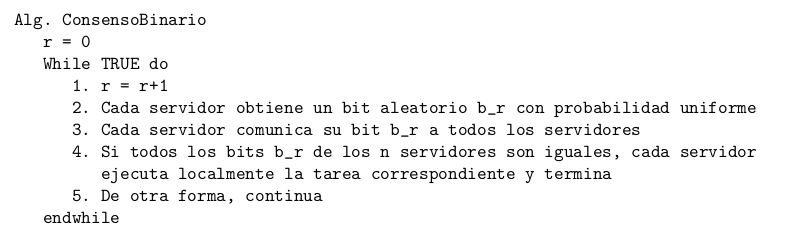
\includegraphics[width=\textwidth]{AlgoProba}
	\end{center}
\end{figure}
\paragraph{Responde a lo siguiente:}
\begin{enumerate}
	\item Demuestra que el número esperado de iteraciones para ejecutar la acción es $O(2^n)$. Tip: Modela el problema con una variable aleatoria con distribución geométrica.
	\item ¿Cuál es el número esperado de iteraciones si en cada una de ellas los servidores obtienen su $r-$ésimo bit, $b_r$, llamando una función \textbf{shared\_random\_bit($r$)} que devuelve el mismo $r-$ésimo bit a todos los servidores con probabilidad $p$, para alguna constante $0 < p < 1$?
\end{enumerate}
\end{document}  